\documentclass[aspectratio=169]{beamer}
\usepackage[utf8]{inputenc}
\usepackage[T1]{fontenc}
\usepackage{amssymb,amsmath,amsthm}
%\usepackage{enumitem}
%\usepackage[osf]{libertine}
\usepackage[mathlf]{MinionPro}
\usepackage{carlito}
\usepackage{inconsolata}
%\usepackage{sectsty}

%\allsectionsfont{\sffamily\mdseries}
\usepackage[tracking=true,spacing=true]{microtype}
\microtypecontext{spacing=nonfrench}
% Set color theme

\newcommand{\proofsep}{\vspace{-0.75em}}
\usepackage{booktabs}

\usepackage{graphicx}
% Improve math spacing around |,\left and \right
% See: https://tex.stackexchange.com/questions/2607/spacing-around-left-and-right/
\let\originalleft\left
\let\originalright\right
\renewcommand{\left}{\mathopen{}\mathclose\bgroup\originalleft}
\renewcommand{\right}{\aftergroup\egroup\originalright}

% Remove section numbering
\makeatletter
% we use \prefix@<level> only if it is defined
\renewcommand{\@seccntformat}[1]{%
	\ifcsname prefix@#1\endcsname
	\csname prefix@#1\endcsname
	\else
	\csname the#1\endcsname\quad
	\fi}
% define \prefix@section
\newcommand\prefix@section{}
\newcommand\prefix@subsection{}
\newcommand\prefix@subsubsection{}
\makeatother

% Define new commands for "such that", the blackboard-bold letters and "closure".
\newcommand{\st}{\textit{ s.t.\ }}
\newcommand{\R}{\ensuremath{\mathbb{R}}}
\newcommand{\N}{\ensuremath{\mathbb{N}}}
\newcommand{\Z}{\ensuremath{\mathbb{Z}}}
\newcommand{\Q}{\ensuremath{\mathbb{Q}}}
\newcommand{\cl}{\ensuremath{\text{cl\hspace{0.1em}}}}
\newcommand{\card}{\ensuremath{\text{card\hspace{0.1em}}}}

\DeclareMathOperator{\blackboardE}{\mathbb{E}}
\newcommand{\expected}[1]{\blackboardE\left[#1\right]}
\newcommand{\expectedwhen}[2]{\blackboardE_{#2}\left[#1\right]}
\newlength{\postparenlength}
\setlength{\postparenlength}{0.14em}
\newcommand{\postparen}{\hspace{\postparenlength}}
\usepackage{url}
\usepackage{xcolor}

\usepackage{siunitx}
\sisetup{
	group-separator={,},
	group-digits = integer,
	input-ignore = {,},
	input-decimal-markers = {.}
}
\usepackage[biblatex]{embrac}

\usepackage[authordate,isbn=false,backend=biber,autopunct=true]{biblatex-chicago}

\addbibresource{refs.bib}


\usetheme{Szeged}
\usecolortheme{dove}
\beamertemplatenavigationsymbolsempty
\title[Cars in Alaska]{EI Research in Progress\\Car Markets and the Alaska Permanent Fund}
\author{Karl Dunkle Werner}
\institute{}
\date{December 12, 2016}
%\usefonttheme{structuresmallcapsserif}
\usefonttheme{serif}


\usepackage[overlay,absolute]{textpos}
\setlength{\TPHorizModule}{\textwidth}
\setlength{\TPVertModule}{\textwidth}

%\usepackage{footnote}
\usepackage{hyperref}
\hypersetup{colorlinks,
	linkcolor=darkgray,
	filecolor=black,
	urlcolor=gray,
	citecolor=darkgray,
	pdfpagemode=UseNone,
	pdftoolbar=false,
	pdftitle={Cohort Presentation -- Alaska Permanent Fund},
	pdfauthor={Karl Dunkle Werner},
	pdfsubject={},
	pdfcreator={},
	pdfproducer={},
	pdflang=en,
	unicode=true
}

\graphicspath{{../../Plots/}}
\begin{document}


% \begin{frame}{To do}
% 	\begin{itemize}
% 		\item Add a photo of Alaska, development style
% 		\item Add some aggregate trend plots
% 		\item Discuss how the dividend check works:
% 		\begin{itemize}
% 			\item Timing of receipt
% 			\item Timing of announcement
% 			\item Payment amount (fixed formula from invested funds, except 2008 and 2016)
% 		\end{itemize}
% 	\end{itemize}
% \end{frame}
% \begin{frame}{Outline}
	% \begin{itemize}
		% \item Cars matter for energy:
		% \begin{itemize}
		% 	\item They're how we consume gasoline
		% 	\item Energy efficiency gap
		% 	\begin{itemize}
		% 		\item Does relaxing income constraint matter for the composition of cars people buy?
		% 		\item Do people treat money from this kind of dividend differently than money from work?
		% 	\end{itemize}
		% \end{itemize}
		% \item And for other questions:
		% \begin{itemize}
		% 	\item Cars are expensive, and important from a pure household economics perspective.
		% 	\item The \textsc{apf} is a relatively rare example of a government taking resource wealth and refunding it directly to citizens -- interesting to see the effects.
		% 	\item Also, from a non-energy perspective, the strongest form of the \textsc{pih} says that we should see no effect in composition or volume of car sales -- maybe interesting. (People have previously used the \textsc{apf} to support the \textsc{pih}, see \cite{hsieh2003})
		% \end{itemize}

% 		\item Acknowledge weakness:
% 		\begin{itemize}
% 			\item Not the best identification
% 			\item The variation I really want, dose--response in the amount of the \textsc{apf} payment, can't be identified separately from macro trends.
% 			\item Only have wholesale car data, which is great for some things and terrible for others.
% 			\begin{itemize}
% 				\item I have to make some assumptions about inventory holding.
% 				\item I have to make some assumptions that dealers in Alaska (i.e. those with Alaskan zip codes) sell their cars to Alaskan people.
% 				\item I don't know anything about the sale to Alaskan people. For example, it would be great to see the prices and composition on that side too.
% 			\end{itemize}
% 		\end{itemize}
% 	\end{itemize}
% \end{frame}

\begin{frame}[plain]
	\maketitle
\end{frame}

{
% full-slide map of alaska
% taken from
% https://commons.wikimedia.org/wiki/File:Alaska_in_United_States_(US50)_(%2Bgrid)_(W3).svg
% Converted with inkscape
\usebackgroundtemplate{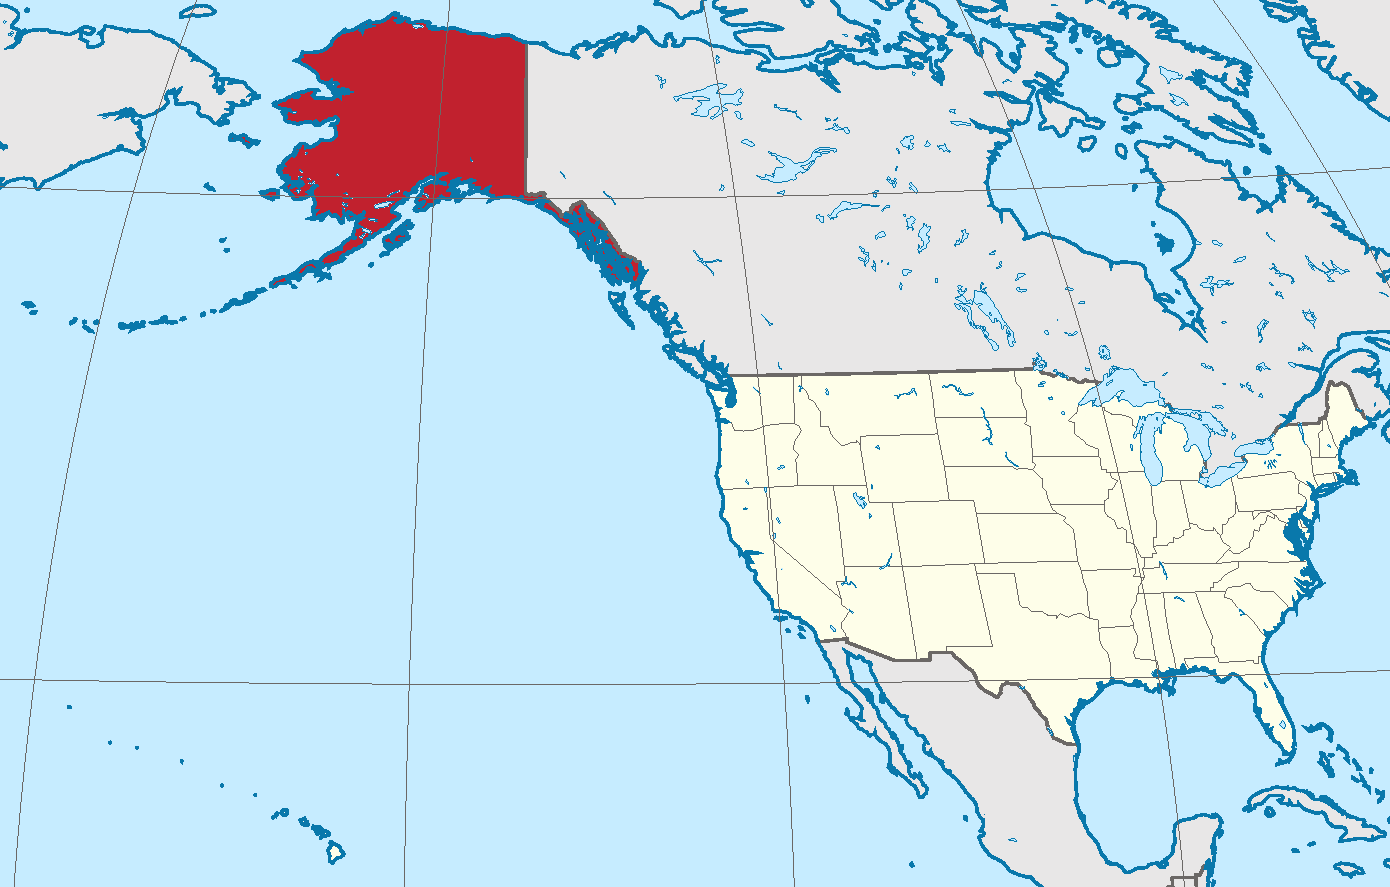
\includegraphics[width=\paperwidth,height=\paperheight]{Alaska_in_United_States_US50_grid_W3.pdf}}
\begin{frame}[plain]
\end{frame}
}


\begin{frame}
	\begin{itemize}
		\item Residents of Alaska get a large check every fall.
	\end{itemize}
	% NOTE Joke here: not enough to buy a fireplace insert, but still a substantial amount of money.
\end{frame}



{  % full-slide plot of the individual payments
\usebackgroundtemplate{\includegraphics{permanent_fund_payments_individual.pdf}}
\begin{frame}[plain]
\end{frame}
}

\begin{frame}
	\begin{itemize}
		\item People in Alaska buy cars.
		\item I observe a large fraction of wholesale used car market sales.
	\end{itemize}
\end{frame}

{  % full-slide plot of the Polk registrations and auction quarterly counts, Alaska vs the rest of the country
\usebackgroundtemplate{
	% \includegraphics{vehicle_registrations_alaska_vs_notitle.pdf}
	\includegraphics{combined_regs_sales_counts_per_capita_alaska_vs_no_resale_quarterly_notitle.pdf}
}
\begin{frame}[plain]
	% NOTE: Some cars are sold multiple times. This graph only includes the last sale of each VIN.
\end{frame}
}
%
% \begin{frame}
%
% 	% Note here: Manheim data, ~50 million sales, 2002-2014.
% 	% TODO: how many sales to Alaskans?
% \end{frame}
%
% {  % full-slide plot of the Manheim auction counts, Alaska vs.
%
% \usebackgroundtemplate{
% 	\includegraphics{auction_sales_counts_per_capita_alaska_vs_no_resale_monthly_qtr_rate_notitle.pdf}
% % NOTE: These are monthly sums of counts, made into quarterly rates by multiplying by 3 (to compare with the quarterly Polk data)
% % NOTE: Some cars are sold multiple times. This graph only includes the last sale of each VIN.
% }
% \begin{frame}[plain]
% \end{frame}
% }

% Outline page
\begin{frame}{Outline}
	\tableofcontents
\end{frame}

\section[Cars]{Why cars?}

\begin{frame}{Why Cars and the APF: Energy}
	\begin{itemize}
		\item They're how we consume gasoline.
		\item Energy efficiency gap:
		\begin{itemize}
			\item Does relaxing income constraint matter for the composition of cars people buy?
			\item Do people treat money from this kind of dividend differently than money from work?
		\end{itemize}
	\end{itemize}
\end{frame}

\begin{frame}{Why Cars and the APF: Non-energy}
	\begin{itemize}
		\item Cars are expensive and economically important.
		\item Refunding resource wealth to citizens.
		% NOTE: The APF is a rare example of a government taking resource wealth and refunding it directly to citizens, which is interesting to examine, even aside from considerations of energy use.
		\item Permanent income hypothesis \parencite{hsieh2003}.
		% NOTE: the strongest form of the PIH says that we should see no effect in composition or volume of car sales -- maybe interesting. (People have previously used the APF to support the PIH, see Hsieh)
	\end{itemize}
\end{frame}


\section[APF Details]{Alaska Permanent Fund details}
% who gets the check?
% what determines how much?
% timing?
\begin{frame}{APF Details}
	\begin{itemize}[<+->]
		\item Fund established in 1976 to hold oil lease revenue.
		\item<.-> Dividends paid in \textsc{q}4 every year since 1984.
		\begin{itemize}
			\item More recently, the first Thursday in October.
		\end{itemize}
		% NOTE: Paid in 1982 and 1983 more erratically
		\item Dividend is 10.5\% of the past five years' investment income, divided evenly.
		\begin{itemize}
			\item<.-> Fund is invested broadly -- think of it as total market returns, not oil profits.
		\end{itemize}
		\item Most people who live in Alaska for at least a year are eligible.
		\begin{itemize}
			\item<.-> \textasciitilde91\% of population applies.
			\item<.-> \textasciitilde95\% of applicants are paid.
		\end{itemize}
		% NOTE: major exception is people convicted of felonies and people serving time.
		\item 2008 bonus (\$2069 $\rightarrow$ \$3269).
		\item<.-> 2016 reduction (\$2052 $\rightarrow$ \$1022; not in my data).
	\end{itemize}
\end{frame}

\section{Research}
\begin{frame}{Research questions}
	% NOTE: Rather than trying to convince you of my very tentative results, I'll run through the
	\begin{itemize}
		\item Quantity effects?
		\item Price effects?
		\begin{itemize}
			\item Paid by Alaskan buyers
			\item Received by Alaskan sellers
			\item For non-Alaskan dealers in states where Alaskan dealers are buying
		\end{itemize}
		\item Composition effects?
		\begin{itemize}
			\item Newness
			% NOTE: newness could be either vehicle age or mileage
			\item Fuel efficiency
			\item Luxury
		\end{itemize}
		\item Dealer anticipation?
	\end{itemize}
\end{frame}
\begin{frame}{Identification: difference-in-differences}
	% Some flavor of difference-in-differences.
	\begin{itemize}
		\item In a window around each dividend payment.
		\begin{itemize}
			\item (Accounting for dealer anticipation)
		\end{itemize}
		\item DD in states where Alaskan buyers are active.
		\item Something fancier, maybe synthetic controls.
	\end{itemize}
\end{frame}
\begin{frame}{Identification assumptions}
	\begin{itemize}
		% NOTE: In any case, I'll need the standard DD assumption; Alaskan car dealers are similar to some appropriately chosen mix of non-Alaskan dealers.
		% NOTE: This is not the strongest identification. Particularly worrying is the concern that seasonal trends in Alaska are dramatically different than in other areas.
		\item Alaskan car dealers are similar to some mix of non-Alaskan dealers.
		\item In particular, there are no seasonal differences within the window I'm examining.
		\item Dose--response in the amount of the \textsc{apf} payment can't be identified separately from macro trends.
		% NOTE: Dose-response in the amount of the APF payment can't be identified separately from macro trends without some aggressive assumptions.
	\end{itemize}
\end{frame}

\section{Data}
\begin{frame}{Data!}
	\begin{itemize}
		\item Manheim wholesale auction data.
		\begin{itemize}
			\item Transaction level, \textasciitilde 50 million sales (8 million resales)
		\end{itemize}
		\item Polk county-by-quarter vehicle registrations.
		\item Consumer expenditure survey.
		% NOTE: the consumer expenditure survey is fine, this isn't what it's designed for.  They don't have many people in Alaska, and the survey weights aren't calculated to give a representative sample at the state level.
		% NOTE: It would certainly be useful to have more fine-grained data on car purchases, but that's the identification is a bigger concern for this project anyway, so I'm not focusing on that.
	\end{itemize}
\end{frame}

\begin{frame}{Next steps}
	\begin{itemize}
		\item Price, quantity and composition effects.
		\item Dealer anticipation.
		\item Consumer side?
	\end{itemize}
\end{frame}
\begin{frame}
\LARGE Questions?
\end{frame}

% \begin{frame}{Data I'd like}
% 	\begin{itemize}
% 		\item Customer car purchases
% 		\item Dealer inventories
% 	\end{itemize}
% \end{frame}
% 	\item Only have wholesale car data, which is great for some things and terrible for others.
% 	\begin{itemize}
% 		\item I have to make some assumptions about inventory holding.
% 		\item I have to make some assumptions that dealers in Alaska (i.e. those with Alaskan zip codes) sell their cars to Alaskan people.
% 		\item I don't know anything about the sale to Alaskan people. For example, it would be great to see the prices and composition on that side too.
% 	\end{itemize}
% \end{itemize}
% \end{itemize}
% \end{frame}



% {
% \usebackgroundtemplate{\includegraphics[width=\paperwidth,height=\paperheight]{permanent_fund_payments_individual.pdf}}
% \begin{frame}[plain]
% \end{frame}
% }
%
% {
% \usebackgroundtemplate{\includegraphics[width=\paperwidth,height=\paperheight]{permanent_fund_payments_aggregate.pdf}}
% \begin{frame}[plain]
% \end{frame}
% }
%
%
% \begin{frame}{Hsieh (2003)}
% 	\[
% 	\log \left(\frac{ C_h^{\textsc{q4}} }{ C_h^{\textsc{q3}} } \right) = \alpha_1
% 	\frac{ \textit{\textsc{pfd}}_t \times \textit{Family size}_h }{\textit{Family income}_h} + \mathbf{z}_h' \mathbf{\alpha}_2
% 	\]
%
% 	\begin{itemize}
% 		\item Do people smooth their consumption when they get the payment?
% 		\begin{itemize}
% 			\item Measured by log of the ratio of \textsc{q4} to \textsc{q3} consumption.
% 		\end{itemize}
% 		\item Use differences in \textsc{pfd} payout and family size as variation in amount household receives in last quarter of the year.
% 		\begin{itemize}
% 			\item Can't control for both year fixed effects and family size.
% 		\end{itemize}
% 		%\item Also compares Alaska vs.\ rest of US
% 	\end{itemize}
%
% \end{frame}
%
% \section{Outcomes}
% \begin{frame}{Big expenses}
% 	Data I have:
% 	\begin{itemize}
% 		\item County-by-quarter counts of new vehicle registrations
% 		\item Wholesale auto auctions, with buyer's and seller's billing zip code
% 		\item Quarterly consumer expenditure data (\textsc{cex})
% 	\end{itemize}
%
% 	Data I want:
% 	\begin{itemize}
% 		\item Medical expenditures (state-by-day or state-by-week)
% 		\item Debt info?
% 		\item Other stuff?
% 	\end{itemize}
% \end{frame}
%
%
% \section{Methods}
%
% \begin{frame}{Difference in Differences}
% 	Still lots of cleaning to do\ldots
% \end{frame}
%
% {
% \usebackgroundtemplate{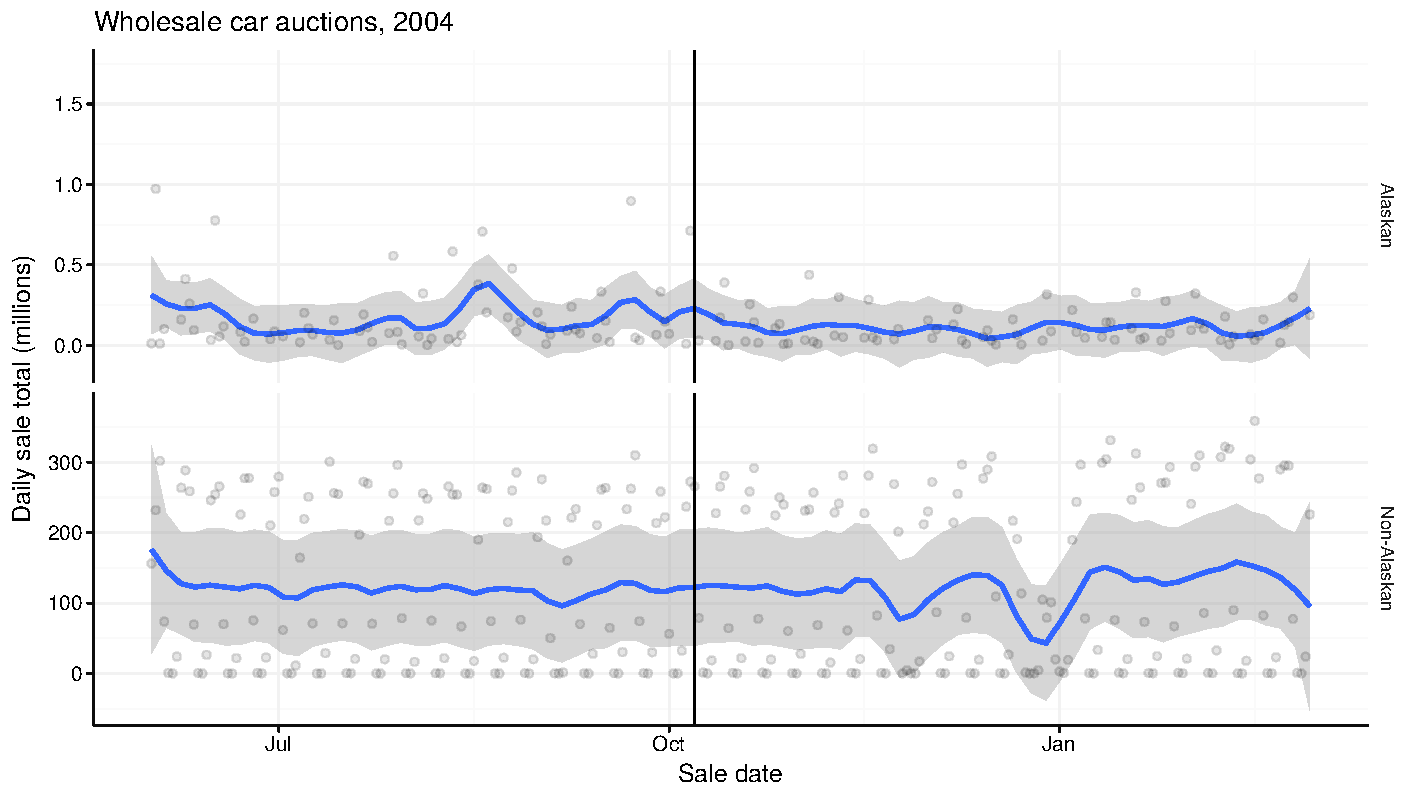
\includegraphics[width=\paperwidth,height=\paperheight]{../../Plots/auctions_2004_alaska_vs_other.pdf}}
% \begin{frame}[plain]
% \end{frame}
% }
%
% \begin{frame}{Synthetic Controls!}
% \end{frame}
%
%
% \begin{frame}{Generalized Synthetic Controls!!}
% 	Synthetic controls, with time-varying factors.
%
% 	Depends on $N\to\infty$ and $T\to\infty$.
% \end{frame}
%
% \begin{frame}{Xu (2016): election-day registration example}
% 	\vspace*{-0.1cm}
% 	\begin{center}
% 		\includegraphics[page=25, trim = 2.5cm 15.5cm 2.0cm 3.0cm, clip,height=7cm]{../../../Papers/Econometrics/Xu_2016.pdf}
% 	\end{center}
% \end{frame}



\end{document}
